% This is samplepaper.tex, a sample chapter demonstrating the
% LLNCS macro package for Springer Computer Science proceedings;
% Version 2.20 of 2017/10/04
%
\documentclass[runningheads]{llncs}
%
\usepackage{graphicx}
% Used for displaying a sample figure. If possible, figure files should
% be included in EPS format.
%
% If you use the hyperref package, please uncomment the following line
% to display URLs in blue roman font according to Springer's eBook style:
% \renewcommand\UrlFont{\color{blue}\rmfamily}

\begin{document}
%
\title{ARQUS Cybersecurity Summer School 2021}
%
%\titlerunning{Abbreviated paper title}
% If the paper title is too long for the running head, you can set
% an abbreviated paper title here
%
\author{Kushagra Singh BISEN\inst{1,2}}
%
\authorrunning{Kushagra Singh BISEN}
% First names are abbreviated in the running head.
% If there are more than two authors, 'et al.' is used.
%
\institute{Universit\'e Jean Monnet, Saint Etienne \and
MINES Saint Etienne, Saint Etienne \\
\email{kushagra.bisen@etu.univ-st-etienne.fr}}
%
\maketitle              % typeset the header of the contribution
%
\begin{abstract}
The document presents the solutions to the challenges given during the ARQUS Cybersecurity summer school held
during 6th to 10th September 2021. The event was hosted by universities located in Italy, France, Lithuania and Spain.
The event promoted collaboration between universities and promoted research across Europe. There are 4 different sections 
detailing each section, concluding with the skills learnt by myself during the course of 4 days.
\keywords{ARQUS  \and Cybersecurity \and Summer-School}
\end{abstract}

\section{Introduction}


\section{Security in Android Applications}
\subsection{Introduction}
Android smartphones are the most popular versions of the modern smartphone. There are around 3 billion 
android smartphones active across the world. By using a popular software, the risk of being exploited by 
unwanted users is tremendously huge. A malware can be used to control/exploit millions of users even if the malware's
reach was not big. Cybersecurity experts, responsible for the security of users plan to tackle the issue in two different ways,
1) Ensuring illegal code practices are not followed. 2) Using analysis tools to check if the application being used is 
safe. During the first day of our security in android application challenge, we were advised to use 
two different tools to analyze the coding practices as well as the security of the application being used. Subsequent sections will describe 
the tools being used and present results from analysis of the tools.

\subsubsection{What is Android?}
Android can be considered an extention to the existing Java JVM library with tools to develop applications.
Android follows a layered architecture \ref{fig1} with application layer containing the applications for the users.
A user never goes further than the application layer, whereas the developers can exploit the other layers based upon the requirement.
Since Android 6.0, Android provides the option for the user to decide if a particular application has the \textbf{permission} 
to use specific resources in the device. Malicious applications try to extract informations by using permissions they do not need but 
use for data mining applications. Android assigns a specific Linux User ID to every application on installation. There are 130 different types of 
permissions an application can ask from the user. They are divided into categories, namely, 1) \textit{Normal}, basic permissions which are automatically granted
by Android. 2) \textit{Dangerous}, permissions required to access important core APIs of Android. 3) \textit{Signature}, permissions which are granted by the developer of the application itself.
4) \textit{SignatureOrSystem}, permissions which granted to the system apps automatically. 
\begin{figure}
    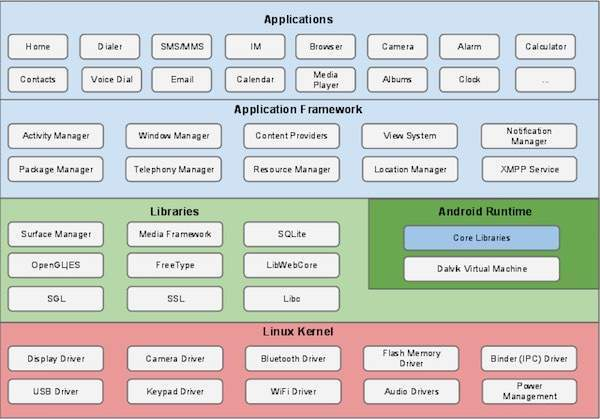
\includegraphics[width=\textwidth]{images/architecture.jpg}
    \caption{The Android OS structure} \label{fig1}
\end{figure}

\subsection{RiskInDroid Analysis Tool}
Analysis of the permissions are usually calculated empirically. An application is judged on a \textit{risk index value} out of 100.
Probabalistic risk index analysis approach for android application is usually a good way to analyze the safety of an application.
RiskInDroid does quantitative risk analysis of android applications which are written in Java. It utilizes machine learning tools such as \textit{scikit-learn}
to generate a numeric risk index value between 0 and 100 for an application. Classifiers such as : \begin{itemize}
    \item Support Vector Machines (SVM)
    \item Multinomial Naive Bayes (MNB)
    \item Gradient Boosting (GB)
    \item Logistic Regression (LR)
\end{itemize}
are employed for classification. 

\textbf{RiskInDroid} takes in consideration both the permissions declares into the applications manifest and the bytecode retreived from the application through 
reverse engineering. Static analysis is used to classify the permissions used in the application into four different ways :
\begin{itemize}
    \item Declared permissions : which are extracted from the application manifest.
    \item Exploited permissions : declared and actually used in the bytecode.
    \item Ghost permissions : not declared but with usages in the bytecode.
    \item Useless permissions : they are declared but not used in the bytecode.
\end{itemize}

The risk value generated is considered to be accurate as it is trained upon 6000 malware samples and 112000 applicaitons of varying levels of security.

\subsubsection{Analysis}
To execute the analysis, we are using : 
\begin{itemize}
    \item Ubuntu 20.04 LTS
    \item Docker 
    \item RiskInDroid Application
    \item Xiaomi Home Application for Analyis
\end{itemize}

\textbf{Instructions} :
\begin{itemize}
    \item git clone \url{https://github.com/ClaudiuGeorgiu/RiskInDroid.git}
    \item docker build -t riskindroid .
    \item docker run --rm -p 8080:80 riskindroid
\end{itemize}

The resulting RiskInDroid application is now running at localhost:8080. \ref{fig2}

\begin{figure}
    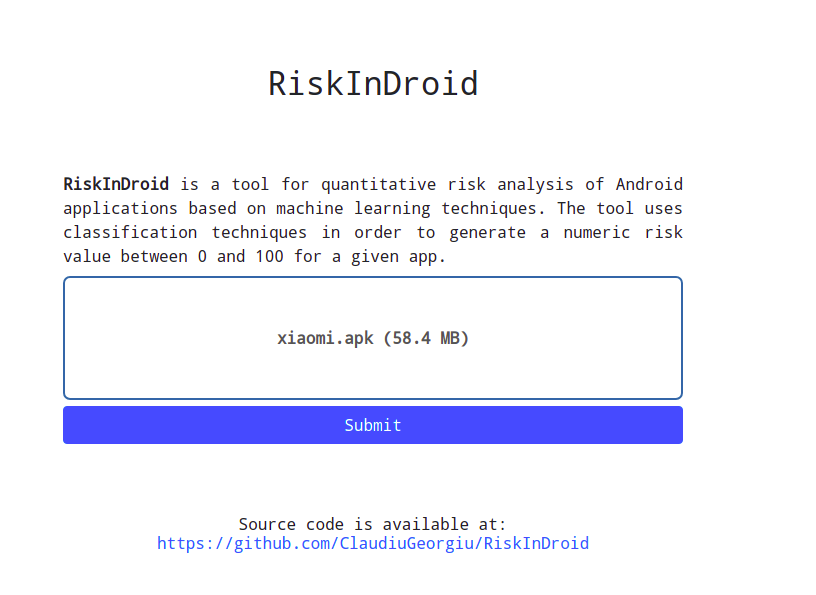
\includegraphics[width=\textwidth]{images/xiaomi-1.png}
    \caption{RiskInDroid Application} \label{fig2}
\end{figure}

\subsubsection{Results}
The Xiaomi application had a score of 30.34. \ref{fig3}.
The results related to permissions were :
\begin{itemize}
    \item Declared - 58 permissions.
    \item Required and Used - 21 permissions.
    \item Required but Not Used - 37 permissions.
    \item Not required but Used - 4 permissions.
\end{itemize}

Developers can use this to analyze the permissions to optimize the use, and thus improving the risk index.

\begin{figure}
    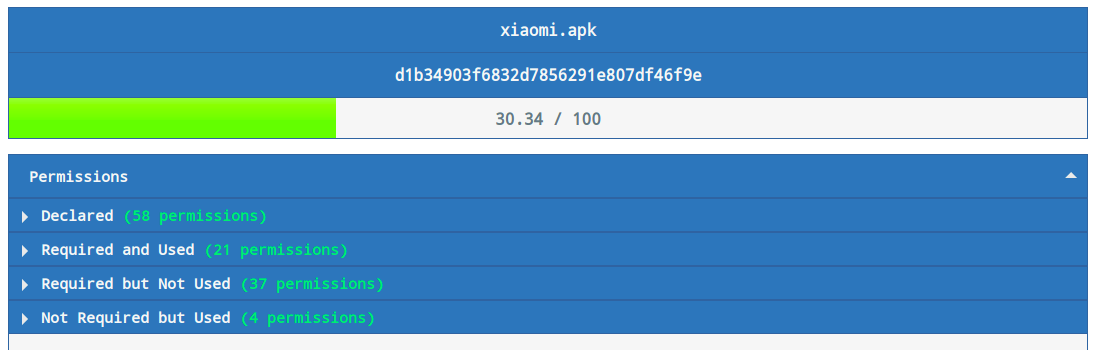
\includegraphics[width=\textwidth]{images/xiaomi-riskinDroid.png}
    \caption{RiskInDroid Application - Xiaomi Analysis} \label{fig3}
\end{figure}


\subsection{SPECK Tool}
As we saw in the previous section, analysis of an application can be done with permissions being provided to the 
android application. One more way to analyze the application is by using the code written to develop the application.
SPECK is a tool designed to search for bad/malicious coding practices in the android application. The software declares a specific set of 
rules to ensure the application's security. 

The many rules divide the intensity of the flaw into three levels : 
\begin{itemize}
    \item \textbf{INFO} : if a good coding practice is detected.
    \item \textbf{WARNING} : if there is an security issue which can be dangerous.
    \item \textbf{CRITICAL} : informs that there is a confirmed security issue.
\end{itemize}

To analyze an android  application, we use the tool in a developer mode. There are 32 different rules which will be used to analyze the coding practices of the android application.
The tools are based upon, 1) Best Practices 2) Security Tips 3) SSL Security 4) Configuration Security 5) Crytography and 6) Direct Boot

The SPECK tool is downloaded and compiled. To analyze the Xiaomi application, we write \textit{python3 Scan.py -s path-to-xiaomi-app}
Manifest and the main java file in analyzed. The application analyzed \textbf{1719} files for the first rule.
In the \ref{fig4}, you see the analysis with Rule 8,9,10 which are : 
\begin{itemize}
    \item Rule 8 : Store private data within internal storage
    \item Rule 9 : Share data securely across apps
    \item Rule 10 : Use scoped directory access
\end{itemize}

A developer can read the output according to the different rules to improve the security of the application. 

\begin{figure}
    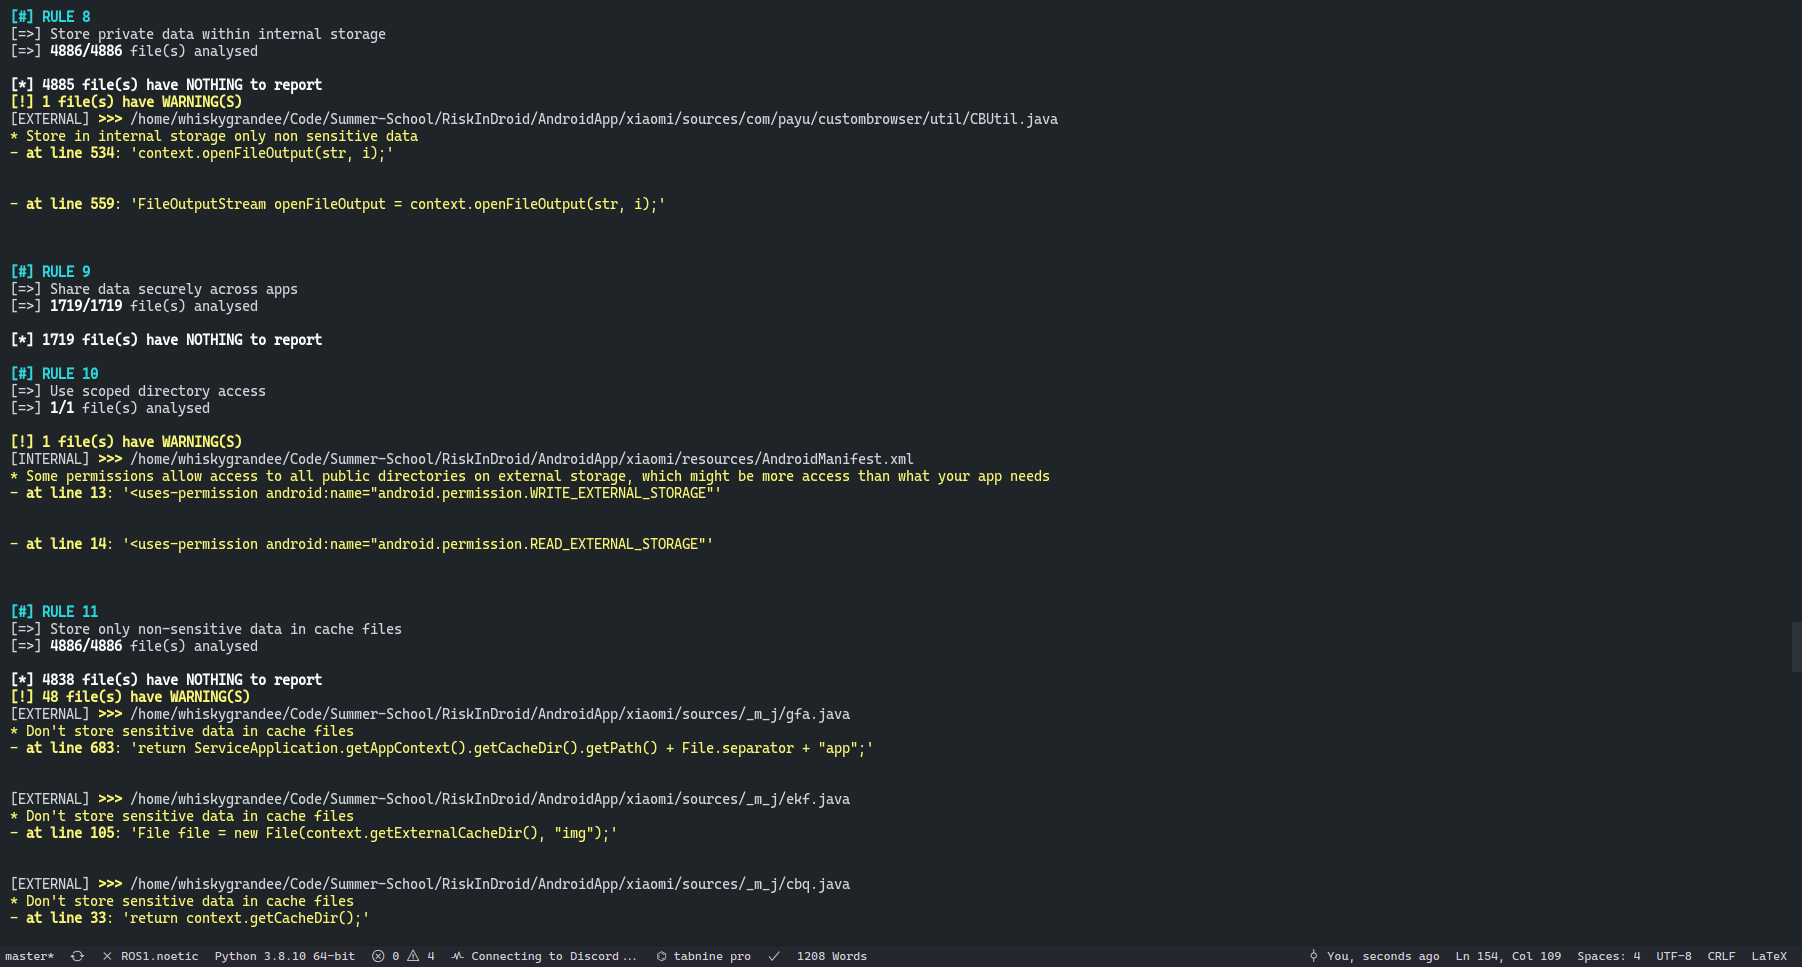
\includegraphics[width=\textwidth]{images/SPECK.png}
    \caption{SPECK Result - Xiaomi Analysis} \label{fig4}
\end{figure}

\section{Buffer Overflow in Cybersecurity}




\section{UNIX commands}

\section{Side Channel Analyis with Deep Learning}

\section{Conclusion}




























%
%
%
\section{First Section}
\subsection{A Subsection Sample}
Please note that the first paragraph of a section or subsection is
not indented. The first paragraph that follows a table, figure,
equation etc. does not need an indent, either.

Subsequent paragraphs, however, are indented.

\subsubsection{Sample Heading (Third Level)} Only two levels of
headings should be numbered. Lower level headings remain unnumbered;
they are formatted as run-in headings.

\paragraph{Sample Heading (Fourth Level)}
The contribution should contain no more than four levels of
headings. Table~\ref{tab1} gives a summary of all heading levels.

\begin{table}
\caption{Table captions should be placed above the
tables.}\label{tab1}
\begin{tabular}{|l|l|l|}
\hline
Heading level &  Example & Font size and style\\
\hline
Title (centered) &  {\Large\bfseries Lecture Notes} & 14 point, bold\\
1st-level heading &  {\large\bfseries 1 Introduction} & 12 point, bold\\
2nd-level heading & {\bfseries 2.1 Printing Area} & 10 point, bold\\
3rd-level heading & {\bfseries Run-in Heading in Bold.} Text follows & 10 point, bold\\
4th-level heading & {\itshape Lowest Level Heading.} Text follows & 10 point, italic\\
\hline
\end{tabular}
\end{table}


\noindent Displayed equations are centered and set on a separate
line.
\begin{equation}
x + y = z
\end{equation}
Please try to avoid rasterized images for line-art diagrams and
schemas. Whenever possible, use vector graphics instead (see
Fig.~\ref{fig1}).

\begin{figure}
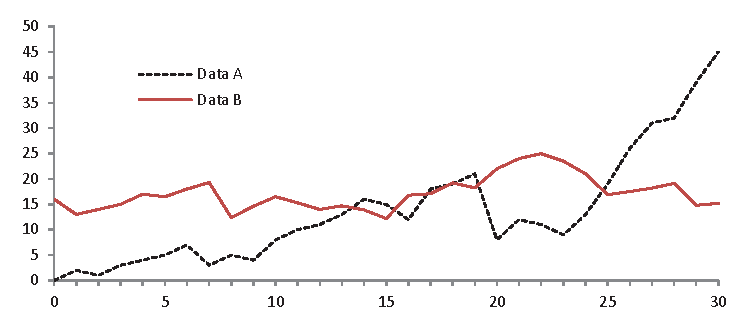
\includegraphics[width=\textwidth]{fig1.eps}
\caption{A figure caption is always placed below the illustration.
Please note that short captions are centered, while long ones are
justified by the macro package automatically.} \label{fig1}
\end{figure}

\begin{theorem}
This is a sample theorem. The run-in heading is set in bold, while
the following text appears in italics. Definitions, lemmas,
propositions, and corollaries are styled the same way.
\end{theorem}
%
% the environments 'definition', 'lemma', 'proposition', 'corollary',
% 'remark', and 'example' are defined in the LLNCS documentclass as well.
%
\begin{proof}
Proofs, examples, and remarks have the initial word in italics,
while the following text appears in normal font.
\end{proof}
For citations of references, we prefer the use of square brackets
and consecutive numbers. Citations using labels or the author/year
convention are also acceptable. The following bibliography provides
a sample reference list with entries for journal
articles~\cite{ref_article1}, an LNCS chapter~\cite{ref_lncs1}, a
book~\cite{ref_book1}, proceedings without editors~\cite{ref_proc1},
and a homepage~\cite{ref_url1}. Multiple citations are grouped
\cite{ref_article1,ref_lncs1,ref_book1},
\cite{ref_article1,ref_book1,ref_proc1,ref_url1}.
%
% ---- Bibliography ----
%
% BibTeX users should specify bibliography style 'splncs04'.
% References will then be sorted and formatted in the correct style.
%
% \bibliographystyle{splncs04}
% \bibliography{mybibliography}
%
\begin{thebibliography}{8}
\bibitem{ref_article1}
Author, F.: Article title. Journal \textbf{2}(5), 99--110 (2016)

\bibitem{ref_lncs1}
Author, F., Author, S.: Title of a proceedings paper. In: Editor,
F., Editor, S. (eds.) CONFERENCE 2016, LNCS, vol. 9999, pp. 1--13.
Springer, Heidelberg (2016). \doi{10.10007/1234567890}

\bibitem{ref_book1}
Author, F., Author, S., Author, T.: Book title. 2nd edn. Publisher,
Location (1999)

\bibitem{ref_proc1}
Author, A.-B.: Contribution title. In: 9th International Proceedings
on Proceedings, pp. 1--2. Publisher, Location (2010)

\bibitem{ref_url1}
LNCS Homepage, \url{http://www.springer.com/lncs}. Last accessed 4
Oct 2017
\end{thebibliography}
\end{document}
